The Reporting Module provides functionality to generate and compare reports
of single/or multiple benchmarks, with the option to export them as pdfs,
whilst still adhearing the quality requirments defined for the system.

\subsection{Architecture Requirements}
\subsubsection{Access and Integration Requirements}
The access requirements for Reporting
\subsubsection{Quality Requirements}
The refined quality requirements for Reporting are discussed below.
\paragraph{Flexibility}
The reporting module should be flexible enough to add different elements,
such as graphs, charts and tables. The color scheme should also be easily
changed. The overall structure of each report should be customizable to each user.
\paragraph{Scalability}
The module should be able to scale with any future scaling of the system.
\paragraph{Performance}
The performance of the reports should as minislistc as possible, such that the
page is responsive as possible.
\paragraph{Reliability}
Each report must be relaible with the data it represents, as this is what the
user will be referring to.
\subsubsection{Architectural Responsibilities}
The architectural responsibilities of the reporting module are shown in
Figure \ref{fig:reportingResponsibilities}
\begin{figure}[H]
	\begin{center}
	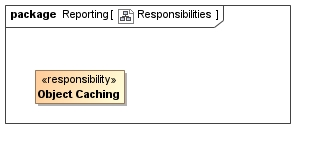
\includegraphics[scale=0.5]{../Diagrams and Charts/Reporting/Responsibilities.jpg}
	\caption{The architectural responsibilities of the Reporting Module}
	\label{fig:reportingResponsibilities}
	\end{center}
\end{figure}
\subsubsection{Architecture Constraints}
The chosen technologies used for the Reporting should be the current active
standard for that technology. With enough documentation available, and community support.

\subsection{Architecture Design}
\subsubsection{Tactics}
The Reporting module should implement the following tactics:
\begin{itemize}
  \item \textit{Report caching} to improve scalability and performance.
\end{itemize}

\subsubsection{Architectural Components}
The architectural components of the Reporting Module are shown in Figure \ref{fig:reportingResponsibilityAllocation}
\begin{figure}[H]
	\begin{center}
	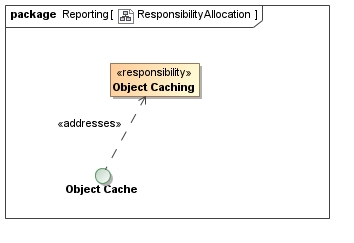
\includegraphics[scale=0.5]{../Diagrams and Charts/Reporting/ResponsibilityAllocation.jpg}
	\caption{The abstract components to which the architectural responsibilities are assigned.}
	\label{fig:reportingResponsibilityAllocation}
	\end{center}
\end{figure}
\subsubsection{Frameworks and Technologies}
The frameworks and technologies used for reporting will consist of javascript,
html and css. With the exporting of reports using a javascript library called jsPDF.

We have considered using the jasper reports to generate reports, but it does
 not provide the full functionality that we are looking for. Such as exporting the graphics of the reports.
